La figure suivante nous montre la porte sur l'intervalle [-32 32] : 
\begin{figure}[H]
\centering
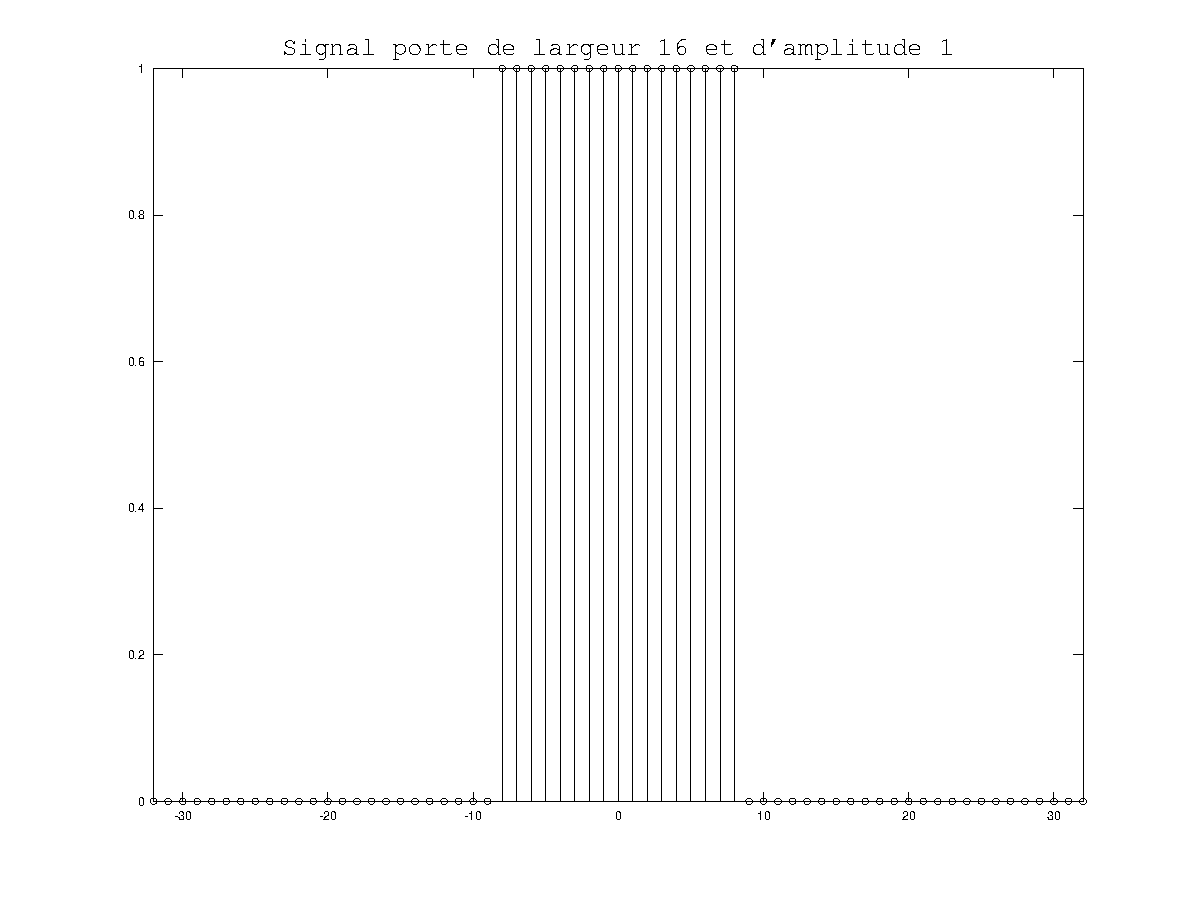
\includegraphics[width=9cm]{resEx1/signalPorte.pdf}
\caption{Signal porte sur l'intervalle [-32 32]}
\end{figure}

La transformé de Fourier de la porte sur l'intervalle [0 0.5] en fréquence réduite donne la courbe ci dessous : 
\begin{figure}[H]
\centering
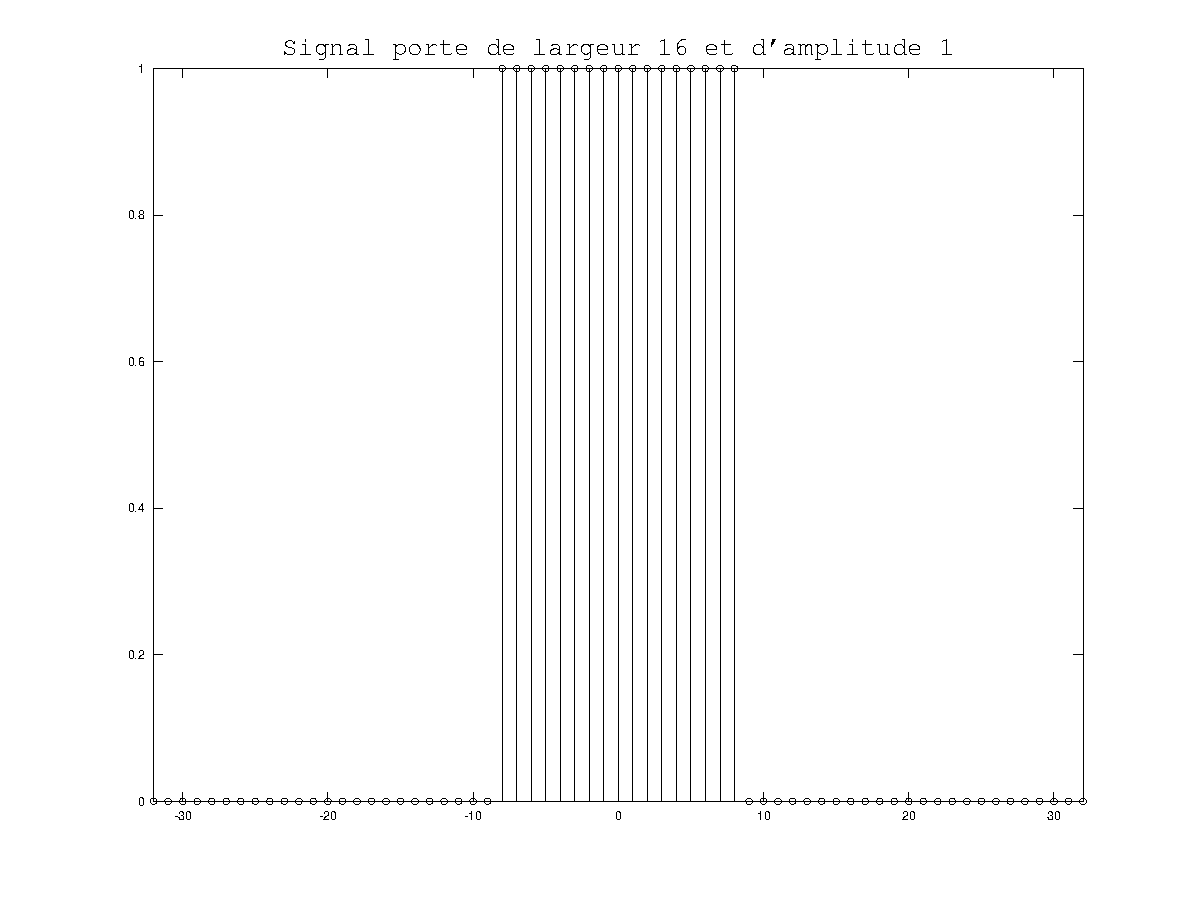
\includegraphics[width=9cm]{resEx1/signalPorte.pdf}
\caption{Signal porte sur l'intervalle [-32 32]}
\end{figure}


